\pdfoutput=1
\documentclass[11pt,a4paper]{article}
\PassOptionsToPackage{linktocpage}{hyperref}
\usepackage[hyperref]{emnlp2018}
\usepackage{times}
\usepackage{latexsym}
\usepackage{todonotes}
\usepackage{amsmath,amssymb}

\usepackage{url}

\usepackage{booktabs}


\usepackage{enumitem}

\newcommand{\relu}{\textsf{relu}}
\newcommand{\lrelua}{\textsf{lrelu-0.01}}
\newcommand{\lrelub}{\textsf{lrelu-0.30}}
\newcommand{\swish}{\textsf{swish}}
\newcommand{\pentan}{\textsf{penalized tanh}}
\newcommand{\arctid}{\textsf{arctid}}
\newcommand{\elu}{\textsf{elu}}
\newcommand{\minsin}{\textsf{minsin}}
\newcommand{\maxtanh}{\textsf{maxtanh}}
\newcommand{\mytanh}{\textsf{tanh}}
\newcommand{\mysin}{\textsf{sin}}
\newcommand{\maxsig}{\textsf{maxsig}}
\newcommand{\selu}{\textsf{selu}}
\newcommand{\linear}{\textsf{linear}}
\newcommand{\sigmoid}{\textsf{sigmoid}}
\newcommand{\cosid}{\textsf{cosid}}
\newcommand{\cube}{\textsf{cube}}
\newcommand{\maxouta}{\textsf{maxout-2}}
\newcommand{\maxoutb}{\textsf{maxout-3}}
\newcommand{\maxoutc}{\textsf{maxout-4}}
\newcommand{\prelu}{\textsf{prelu}}
\newcommand{\best}{\texttt{best}}


\newcommand{\avg}{\texttt{mean}}


\aclfinalcopy
\def\aclpaperid{256}


\newcommand\BibTeX{B{\sc ib}\TeX}
\newcommand\confname{EMNLP 2018}
\newcommand\conforg{SIGDAT}

\title{Is it Time to Swish? \\ Comparing Deep Learning Activation Functions Across NLP tasks}

\author{Steffen Eger, Paul Youssef, Iryna Gurevych \\
  Ubiquitous Knowledge Processing Lab (UKP-TUDA) \\
  Department of Computer Science \\
  Technische Universit\"at Darmstadt\\
  {\tt www.ukp.tu-darmstadt.de}
  }

\date{}

\begin{document}
\maketitle
\begin{abstract}
Activation functions play a crucial role in neural networks because they are the non-linearities which have been attributed to the success story of deep learning. One of the currently most popular activation functions is ReLU, but several competitors have recently been proposed or `discovered', including LReLU functions and \swish. While most works compare newly proposed activation functions on few tasks (usually from image classification) and against few competitors (usually ReLU), we perform the first large-scale comparison of 21 activation functions across eight different NLP tasks. We find that a largely unknown activation function performs most stably across all tasks, the so-called \pentan{} function. We also show that it can successfully replace the \sigmoid{} and \mytanh{} gates in LSTM cells, leading to a 2 percentage point (pp) improvement over the standard choices on a challenging NLP task.
\end{abstract}

\section{Introduction}

\section{Theory}

\paragraph{Activation functions}

\begin{table}[!htb]
  \centering
  \begin{tabular}{ll}
  \toprule
    \sigmoid & $f(x)=\sigma(x)=1/(1+\exp(-x))$\\
    \swish & $f(x)=x\cdot \sigma(x)$\\
    \maxsig & $f(x)=\max\{x,\sigma(x)\}$\\
    \cosid & $f(x)=\cos(x)-x$\\
    \minsin & $f(x)=\min\{x,\sin(x)\}$\\
    \arctid & $f(x)=\arctan(x)^2-x$\\
    \maxtanh & $f(x)=\max\{x,\tanh(x)\}$\\
    \midrule
    \lrelua & $f(x)=\max\{x,0.01x\}$ \\
    \lrelub & $f(x)=\max\{x,0.3x\}$ \\
    {\small \pentan} & $f(x)=\begin{cases}\tanh(x) & x>0,\\ 0.25\tanh(x) & x\le 0\end{cases}$\\
    \bottomrule
  \end{tabular}
  \caption{Top: \sigmoid{} activation function as well as 6 top performing activation functions from \citet{Ramach:2018}. Bottom: the LReLU functions with different parametrizations as well as \pentan{}.}
  \label{table:functions}
\end{table}

\paragraph{Properties of activation functions}

\begin{table*}[!htb]
\centering
\footnotesize
\begin{tabular}{llll}
  \toprule
  Property & Description & Problems & Examples \\ \midrule
  derivative & $f'$ & $>1$ exploding gradient (e) &  \sigmoid{} (v), \mytanh{} (v), \cube{} (e)\\
  & & $<1$ vanishing (v) & \\
  zero-centered & range centered around zero? &   if not, slower learning & \mytanh{} ($+$), \relu{} ($-$) \\
  saturating & finite limits & vanishing gradient in the limit & \mytanh{}, \pentan{}, \sigmoid{}\\
  monotonicity & $x>y\implies f(x)\ge f(y)$ & unclear & exceptions: \mysin{}, \swish{}, \minsin{}
  \\ \bottomrule
 \end{tabular}
 \caption{Frequently cited properties of activation functions}.
 \label{table:properties}
\end{table*}

\section{Experiments}

\subsection{MLP \& Sentence Classification}

\paragraph{Model}

\begin{align*}
  \mathbf{x}_i &= f(\mathbf{x}_{i-1}\cdot \mathbf{W}_i+\mathbf{b}_i)\\
  \mathbf{y} &= \text{softmax}(\mathbf{x}_{N}\mathbf{W}_{N+1}+\mathbf{b}_{N+1})
\end{align*}

\paragraph{Data}

\begin{table*}[!htb]
\centering
%\footnotesize
\small
\begin{tabular}{llccll}
\toprule
\textbf{Task} & \textbf{Type} & \textbf{Size} & \textbf{C} & \textbf{Example} \\ 
\midrule
{AM} & Argumentation & 7k  & 4 &
Not cooking fresh food will lead to lack of nutrition. \textit{(claim)} 
 \\
{MR} & Sentiment & 11k & 2 & Too slow for a younger crowd , too shallow for an older one. \textit{(neg)} \\
{SUBJ} & Subjectivity & 10k & 2 & A movie that doesn’t aim too high , but doesn’t need to. \textit{(subj)} \\
{TREC} & Question-types & 6k & 6 & What's the Olympic Motto? \textit{(description)} \\
\midrule
NG & Doc classification & 18k & 20 & [...] You can add "dark matter" and quarks [...] (\emph{sci.space})\\
R8 & Doc classification & 7k & 8 & bowater industries profit exceed [...] (\emph{earn})\\
\midrule
POS & POS tagging & 204k & 17 & What/\emph{PRON} to/\emph{PART} feed/\emph{VERB} my/\emph{PRON} dog/\emph{NOUN} [...]\\
TL-AM & Token-level AM & 148k & 7 & [...] I/\emph{O} firmly/\emph{O} believe/\emph{O} that/\emph{O} we/\emph{B-MC} should/\emph{I-MC} [...]\\
\bottomrule
\end{tabular}
\caption{Evaluation tasks used in our experiments, grouped by task type (sentence classification, document classification, sequence tagging), with statistics and examples. C is the number of classes to predict.}
\label{table:data_sent}
\end{table*}

\paragraph{Approach}

\begin{itemize}[noitemsep,leftmargin=0.6cm]
  \item (1): MR dataset with Sent2Vec-unigram embeddings as input and 1\% of the full data as training data; (2): the same mini-experiment with 50\% of the full data as training data. In both cases, the dev set comprises 10\% of the full data and the rest is for testing.
  \item (3,4): SUBJ with InferSent embeddings and likewise 1\% and 50\% of the full data as train data, respectively.
  \item (5): The TREC dataset with original split in train and test; 50\% of the train split is used as dev data.
  \item (6): The AM dataset with original split in train, dev, and test \cite{Eger:2017}, and with InferSent input embeddings. (7): the same mini-experiment with Sent2Vec-unigram embeddings.
\end{itemize}

\begin{table*}[htb]
  \centering
  {\small
  \begin{tabular}{llr}
  \toprule
    Model & Hyperparameter & Range \\ \toprule
    %InferSent$+$MLP & & \\
    (a) MLP & (1) optimizer & $\{$Adam,RMSprop,Adagrad,Adadelta,Adamax,Nadam,sgd$\}$ \\
    & (2) \#hidden layers $N$ & $\{1,2,3,4\}$\\
    & (3) dropout value & $[0.1,0.75]$ \\
    %(a) MLP 
    & (4) hidden units & $[30,500]$ \\
    & (5) learning rate & $\mathcal{N}(m,m/5)$\\
    & (6) weight initializer & $\{$random-n, random-u, varscaling, orthogonal, \\
    & & lecun-u, glorot-n, glorot-u, he-n, he-u$\}$\\
    \midrule
    %FastText & & \\
             %& minCount & $\{0,1,2\}$\\
     (b) CNN        & (a) (1,3,5,6) & same as MLP \\
             %& epochs & $\{500,1000,2000\}$ \\
             & embedding dimension & $[40,200]$\\
     %(b) CNN        
     & number of filters $n_k$ & $[30,500]$\\
             & \#hidden layers $N$ & $\{1,2,3\}$\\
             & filter size $h$ & $\{1,2,2,3,3,3,4\}$\\
%     & hidden size & $\{50,75,100,125,150,200,300,500\}$\\
%    \HAN & embedding size &  $\{50,100,150,200,300,400,500\}$ \\
  %  & devsize & $\{0.1,0.2,0.3,0.4\}$\\
%    & pretrained word vectors & $\{\text{None},\text{Komninos},\text{Glove}\}$\\
    %& regularization coefficient &  $[0.01, 10]$ \\
    \midrule
      (c) RNN/LSTM & (a) (1-5) & same as MLP \\
     & recurrent initializer & same as (a) (6) plus identity matrix\\
    %& & $\{31,32,33,34,35,36,37,38,39,40\}$ \\
    \midrule
  \end{tabular}
  \caption{Hyperparameter ranges for each network type. Hyperparameters are drawn using a discrete or continuous uniform distribution from the indicated ranges. Repeated values indicate multi-sets. $\mathcal{N}(\mu,s)$ is the normal distribution with mean $\mu$ and std $s$; $\mu=m$ is the default value from keras for the specific optimizer (if drawn learning rate is $<0$, we choose it to be $m$).}
  \label{table:hyperparams_sent}
  }
\end{table*}

\paragraph{Results}

\begin{figure}[htb]
  \centering
  \scalebox{0.5}{% GNUPLOT: LaTeX picture with Postscript
\begingroup
  \makeatletter
  \providecommand\color[2][]{%
    \GenericError{(gnuplot) \space\space\space\@spaces}{%
      Package color not loaded in conjunction with
      terminal option `colourtext'%
    }{See the gnuplot documentation for explanation.%
    }{Either use 'blacktext' in gnuplot or load the package
      color.sty in LaTeX.}%
    \renewcommand\color[2][]{}%
  }%
  \providecommand\includegraphics[2][]{%
    \GenericError{(gnuplot) \space\space\space\@spaces}{%
      Package graphicx or graphics not loaded%
    }{See the gnuplot documentation for explanation.%
    }{The gnuplot epslatex terminal needs graphicx.sty or graphics.sty.}%
    \renewcommand\includegraphics[2][]{}%
  }%
  \providecommand\rotatebox[2]{#2}%
  \@ifundefined{ifGPcolor}{%
    \newif\ifGPcolor
    \GPcolortrue
  }{}%
  \@ifundefined{ifGPblacktext}{%
    \newif\ifGPblacktext
    \GPblacktexttrue
  }{}%
  % define a \g@addto@macro without @ in the name:
  \let\gplgaddtomacro\g@addto@macro
  % define empty templates for all commands taking text:
  \gdef\gplbacktext{}%
  \gdef\gplfronttext{}%
  \makeatother
  \ifGPblacktext
    % no textcolor at all
    \def\colorrgb#1{}%
    \def\colorgray#1{}%
  \else
    % gray or color?
    \ifGPcolor
      \def\colorrgb#1{\color[rgb]{#1}}%
      \def\colorgray#1{\color[gray]{#1}}%
      \expandafter\def\csname LTw\endcsname{\color{white}}%
      \expandafter\def\csname LTb\endcsname{\color{black}}%
      \expandafter\def\csname LTa\endcsname{\color{black}}%
      \expandafter\def\csname LT0\endcsname{\color[rgb]{1,0,0}}%
      \expandafter\def\csname LT1\endcsname{\color[rgb]{0,1,0}}%
      \expandafter\def\csname LT2\endcsname{\color[rgb]{0,0,1}}%
      \expandafter\def\csname LT3\endcsname{\color[rgb]{1,0,1}}%
      \expandafter\def\csname LT4\endcsname{\color[rgb]{0,1,1}}%
      \expandafter\def\csname LT5\endcsname{\color[rgb]{1,1,0}}%
      \expandafter\def\csname LT6\endcsname{\color[rgb]{0,0,0}}%
      \expandafter\def\csname LT7\endcsname{\color[rgb]{1,0.3,0}}%
      \expandafter\def\csname LT8\endcsname{\color[rgb]{0.5,0.5,0.5}}%
    \else
      % gray
      \def\colorrgb#1{\color{black}}%
      \def\colorgray#1{\color[gray]{#1}}%
      \expandafter\def\csname LTw\endcsname{\color{white}}%
      \expandafter\def\csname LTb\endcsname{\color{black}}%
      \expandafter\def\csname LTa\endcsname{\color{black}}%
      \expandafter\def\csname LT0\endcsname{\color{black}}%
      \expandafter\def\csname LT1\endcsname{\color{black}}%
      \expandafter\def\csname LT2\endcsname{\color{black}}%
      \expandafter\def\csname LT3\endcsname{\color{black}}%
      \expandafter\def\csname LT4\endcsname{\color{black}}%
      \expandafter\def\csname LT5\endcsname{\color{black}}%
      \expandafter\def\csname LT6\endcsname{\color{black}}%
      \expandafter\def\csname LT7\endcsname{\color{black}}%
      \expandafter\def\csname LT8\endcsname{\color{black}}%
    \fi
  \fi
  \setlength{\unitlength}{0.0500bp}%
  \begin{picture}(8502.00,6802.00)%
    \gplgaddtomacro\gplbacktext{%
      \csname LTb\endcsname%
      \put(784,2001){\makebox(0,0)[r]{\strut{} 98}}%
      \csname LTb\endcsname%
      \put(784,3153){\makebox(0,0)[r]{\strut{} 98.5}}%
      \csname LTb\endcsname%
      \put(784,4305){\makebox(0,0)[r]{\strut{} 99}}%
      \csname LTb\endcsname%
      \put(784,5457){\makebox(0,0)[r]{\strut{} 99.5}}%
      \csname LTb\endcsname%
      \put(784,6609){\makebox(0,0)[r]{\strut{} 100}}%
      \csname LTb\endcsname%
      \put(880,1408){\rotatebox{-270}{\makebox(0,0)[r]{\strut{}\relu}}}%
      \csname LTb\endcsname%
      \put(1223,1408){\rotatebox{-270}{\makebox(0,0)[r]{\strut{}\lrelua}}}%
      \csname LTb\endcsname%
      \put(1565,1408){\rotatebox{-270}{\makebox(0,0)[r]{\strut{}\maxoutc}}}%
      \csname LTb\endcsname%
      \put(1908,1408){\rotatebox{-270}{\makebox(0,0)[r]{\strut{}\maxoutb}}}%
      \csname LTb\endcsname%
      \put(2251,1408){\rotatebox{-270}{\makebox(0,0)[r]{\strut{}\pentan}}}%
      \csname LTb\endcsname%
      \put(2593,1408){\rotatebox{-270}{\makebox(0,0)[r]{\strut{}\prelu}}}%
      \csname LTb\endcsname%
      \put(2936,1408){\rotatebox{-270}{\makebox(0,0)[r]{\strut{}\maxouta}}}%
      \csname LTb\endcsname%
      \put(3279,1408){\rotatebox{-270}{\makebox(0,0)[r]{\strut{}\minsin}}}%
      \csname LTb\endcsname%
      \put(3621,1408){\rotatebox{-270}{\makebox(0,0)[r]{\strut{}\swish}}}%
      \csname LTb\endcsname%
      \put(3964,1408){\rotatebox{-270}{\makebox(0,0)[r]{\strut{}\mytanh}}}%
      \csname LTb\endcsname%
      \put(4307,1408){\rotatebox{-270}{\makebox(0,0)[r]{\strut{}\selu}}}%
      \csname LTb\endcsname%
      \put(4649,1408){\rotatebox{-270}{\makebox(0,0)[r]{\strut{}\mysin}}}%
      \csname LTb\endcsname%
      \put(4992,1408){\rotatebox{-270}{\makebox(0,0)[r]{\strut{}\lrelub}}}%
      \csname LTb\endcsname%
      \put(5334,1408){\rotatebox{-270}{\makebox(0,0)[r]{\strut{}\maxsig}}}%
      \csname LTb\endcsname%
      \put(5677,1408){\rotatebox{-270}{\makebox(0,0)[r]{\strut{}\maxtanh}}}%
      \csname LTb\endcsname%
      \put(6020,1408){\rotatebox{-270}{\makebox(0,0)[r]{\strut{}\cosid}}}%
      \csname LTb\endcsname%
      \put(6362,1408){\rotatebox{-270}{\makebox(0,0)[r]{\strut{}\cube}}}%
      \csname LTb\endcsname%
      \put(6705,1408){\rotatebox{-270}{\makebox(0,0)[r]{\strut{}\sigmoid}}}%
      \csname LTb\endcsname%
      \put(7048,1408){\rotatebox{-270}{\makebox(0,0)[r]{\strut{}\arctid}}}%
      \csname LTb\endcsname%
      \put(7390,1408){\rotatebox{-270}{\makebox(0,0)[r]{\strut{}\elu}}}%
      \csname LTb\endcsname%
      \put(7733,1408){\rotatebox{-270}{\makebox(0,0)[r]{\strut{}\linear}}}%
      \put(7829,2103){\makebox(0,0)[l]{\strut{} 69}}%
      \put(7829,2830){\makebox(0,0)[l]{\strut{} 74}}%
      \put(7829,3557){\makebox(0,0)[l]{\strut{} 79}}%
      \put(7829,4284){\makebox(0,0)[l]{\strut{} 84}}%
      \put(7829,5010){\makebox(0,0)[l]{\strut{} 89}}%
      \put(7829,5737){\makebox(0,0)[l]{\strut{} 94}}%
      \put(7829,6464){\makebox(0,0)[l]{\strut{} 99}}%
      \put(128,4056){\rotatebox{-270}{\makebox(0,0){\strut{}Score}}}%
    }%
    \gplgaddtomacro\gplfronttext{%
      \csname LTb\endcsname%
      \put(6998,6466){\makebox(0,0)[r]{\strut{}\best{}}}%
      \csname LTb\endcsname%
      \put(6998,6306){\makebox(0,0)[r]{\strut{}\avg{}}}%
    }%
    \gplbacktext
    \put(0,0){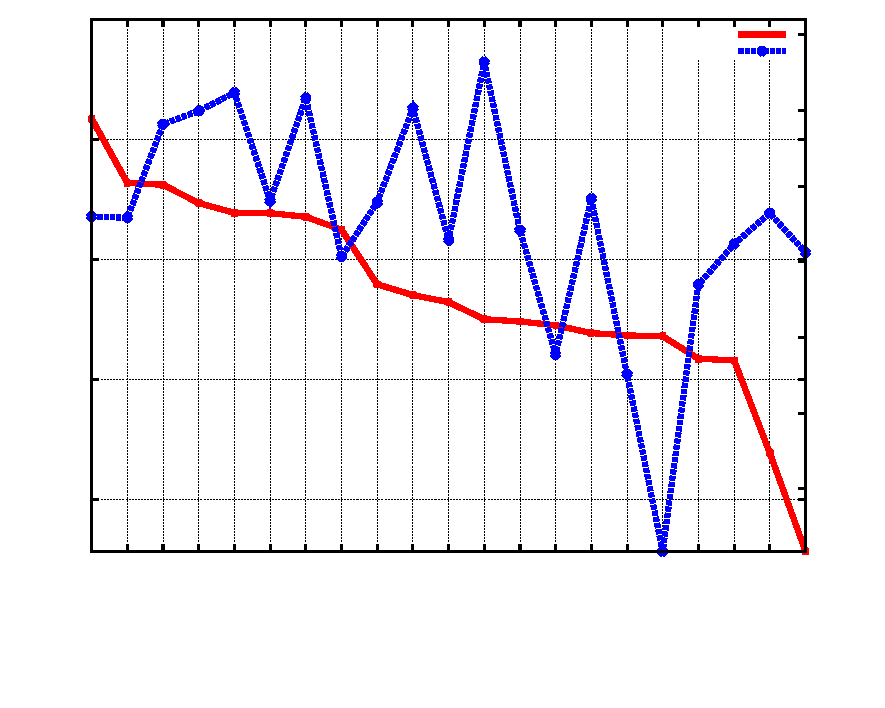
\includegraphics{plots/sent-X.pdf}}%
    \gplfronttext
  \end{picture}%
\endgroup
}
  \caption{Sentence Classification. Left y-axis: \best. Right y-axis: \avg{}. Score on y-axes is the average over all mini-experiments.}
  \label{fig:sent}
\end{figure}

\subsection{CNN \& Document Classification}

\paragraph{Model}

\begin{align*}
  c_i = f(\mathbf{w}\cdot \mathbf{x}_{i:i+h-1}+b).
\end{align*}

\paragraph{Data}

\paragraph{Approach}

\begin{itemize}[noitemsep,leftmargin=0.6cm]
\item (1,2) NG dataset with 5\% and 50\%, respectively of the full data as train data. In both cases, 10\% of the full data is used as dev data, and the rest as test data.
\item (3,4) Same as (1,2) for R8.
\end{itemize}

\paragraph{Results}

\begin{figure}[!htb]
\centering
\scalebox{0.5}{% GNUPLOT: LaTeX picture with Postscript
\begingroup
  \makeatletter
  \providecommand\color[2][]{%
    \GenericError{(gnuplot) \space\space\space\@spaces}{%
      Package color not loaded in conjunction with
      terminal option `colourtext'%
    }{See the gnuplot documentation for explanation.%
    }{Either use 'blacktext' in gnuplot or load the package
      color.sty in LaTeX.}%
    \renewcommand\color[2][]{}%
  }%
  \providecommand\includegraphics[2][]{%
    \GenericError{(gnuplot) \space\space\space\@spaces}{%
      Package graphicx or graphics not loaded%
    }{See the gnuplot documentation for explanation.%
    }{The gnuplot epslatex terminal needs graphicx.sty or graphics.sty.}%
    \renewcommand\includegraphics[2][]{}%
  }%
  \providecommand\rotatebox[2]{#2}%
  \@ifundefined{ifGPcolor}{%
    \newif\ifGPcolor
    \GPcolortrue
  }{}%
  \@ifundefined{ifGPblacktext}{%
    \newif\ifGPblacktext
    \GPblacktexttrue
  }{}%
  % define a \g@addto@macro without @ in the name:
  \let\gplgaddtomacro\g@addto@macro
  % define empty templates for all commands taking text:
  \gdef\gplbacktext{}%
  \gdef\gplfronttext{}%
  \makeatother
  \ifGPblacktext
    % no textcolor at all
    \def\colorrgb#1{}%
    \def\colorgray#1{}%
  \else
    % gray or color?
    \ifGPcolor
      \def\colorrgb#1{\color[rgb]{#1}}%
      \def\colorgray#1{\color[gray]{#1}}%
      \expandafter\def\csname LTw\endcsname{\color{white}}%
      \expandafter\def\csname LTb\endcsname{\color{black}}%
      \expandafter\def\csname LTa\endcsname{\color{black}}%
      \expandafter\def\csname LT0\endcsname{\color[rgb]{1,0,0}}%
      \expandafter\def\csname LT1\endcsname{\color[rgb]{0,1,0}}%
      \expandafter\def\csname LT2\endcsname{\color[rgb]{0,0,1}}%
      \expandafter\def\csname LT3\endcsname{\color[rgb]{1,0,1}}%
      \expandafter\def\csname LT4\endcsname{\color[rgb]{0,1,1}}%
      \expandafter\def\csname LT5\endcsname{\color[rgb]{1,1,0}}%
      \expandafter\def\csname LT6\endcsname{\color[rgb]{0,0,0}}%
      \expandafter\def\csname LT7\endcsname{\color[rgb]{1,0.3,0}}%
      \expandafter\def\csname LT8\endcsname{\color[rgb]{0.5,0.5,0.5}}%
    \else
      % gray
      \def\colorrgb#1{\color{black}}%
      \def\colorgray#1{\color[gray]{#1}}%
      \expandafter\def\csname LTw\endcsname{\color{white}}%
      \expandafter\def\csname LTb\endcsname{\color{black}}%
      \expandafter\def\csname LTa\endcsname{\color{black}}%
      \expandafter\def\csname LT0\endcsname{\color{black}}%
      \expandafter\def\csname LT1\endcsname{\color{black}}%
      \expandafter\def\csname LT2\endcsname{\color{black}}%
      \expandafter\def\csname LT3\endcsname{\color{black}}%
      \expandafter\def\csname LT4\endcsname{\color{black}}%
      \expandafter\def\csname LT5\endcsname{\color{black}}%
      \expandafter\def\csname LT6\endcsname{\color{black}}%
      \expandafter\def\csname LT7\endcsname{\color{black}}%
      \expandafter\def\csname LT8\endcsname{\color{black}}%
    \fi
  \fi
  \setlength{\unitlength}{0.0500bp}%
  \begin{picture}(8502.00,6802.00)%
    \gplgaddtomacro\gplbacktext{%
      \csname LTb\endcsname%
      \put(784,1551){\makebox(0,0)[r]{\strut{} 94.5}}%
      \csname LTb\endcsname%
      \put(784,2010){\makebox(0,0)[r]{\strut{} 95}}%
      \csname LTb\endcsname%
      \put(784,2470){\makebox(0,0)[r]{\strut{} 95.5}}%
      \csname LTb\endcsname%
      \put(784,2930){\makebox(0,0)[r]{\strut{} 96}}%
      \csname LTb\endcsname%
      \put(784,3390){\makebox(0,0)[r]{\strut{} 96.5}}%
      \csname LTb\endcsname%
      \put(784,3850){\makebox(0,0)[r]{\strut{} 97}}%
      \csname LTb\endcsname%
      \put(784,4310){\makebox(0,0)[r]{\strut{} 97.5}}%
      \csname LTb\endcsname%
      \put(784,4770){\makebox(0,0)[r]{\strut{} 98}}%
      \csname LTb\endcsname%
      \put(784,5229){\makebox(0,0)[r]{\strut{} 98.5}}%
      \csname LTb\endcsname%
      \put(784,5689){\makebox(0,0)[r]{\strut{} 99}}%
      \csname LTb\endcsname%
      \put(784,6149){\makebox(0,0)[r]{\strut{} 99.5}}%
      \csname LTb\endcsname%
      \put(784,6609){\makebox(0,0)[r]{\strut{} 100}}%
      \csname LTb\endcsname%
      \put(880,1408){\rotatebox{-270}{\makebox(0,0)[r]{\strut{}\elu}}}%
      \csname LTb\endcsname%
      \put(1218,1408){\rotatebox{-270}{\makebox(0,0)[r]{\strut{}\selu}}}%
      \csname LTb\endcsname%
      \put(1556,1408){\rotatebox{-270}{\makebox(0,0)[r]{\strut{}\maxouta}}}%
      \csname LTb\endcsname%
      \put(1894,1408){\rotatebox{-270}{\makebox(0,0)[r]{\strut{}\mytanh}}}%
      \csname LTb\endcsname%
      \put(2231,1408){\rotatebox{-270}{\makebox(0,0)[r]{\strut{}\minsin}}}%
      \csname LTb\endcsname%
      \put(2569,1408){\rotatebox{-270}{\makebox(0,0)[r]{\strut{}\pentan}}}%
      \csname LTb\endcsname%
      \put(2907,1408){\rotatebox{-270}{\makebox(0,0)[r]{\strut{}\maxoutb}}}%
      \csname LTb\endcsname%
      \put(3245,1408){\rotatebox{-270}{\makebox(0,0)[r]{\strut{}\mysin}}}%
      \csname LTb\endcsname%
      \put(3583,1408){\rotatebox{-270}{\makebox(0,0)[r]{\strut{}\maxoutc}}}%
      \csname LTb\endcsname%
      \put(3921,1408){\rotatebox{-270}{\makebox(0,0)[r]{\strut{}\prelu}}}%
      \csname LTb\endcsname%
      \put(4259,1408){\rotatebox{-270}{\makebox(0,0)[r]{\strut{}\linear}}}%
      \csname LTb\endcsname%
      \put(4596,1408){\rotatebox{-270}{\makebox(0,0)[r]{\strut{}\lrelub}}}%
      \csname LTb\endcsname%
      \put(4934,1408){\rotatebox{-270}{\makebox(0,0)[r]{\strut{}\maxtanh}}}%
      \csname LTb\endcsname%
      \put(5272,1408){\rotatebox{-270}{\makebox(0,0)[r]{\strut{}\lrelua}}}%
      \csname LTb\endcsname%
      \put(5610,1408){\rotatebox{-270}{\makebox(0,0)[r]{\strut{}\relu}}}%
      \csname LTb\endcsname%
      \put(5948,1408){\rotatebox{-270}{\makebox(0,0)[r]{\strut{}\arctid}}}%
      \csname LTb\endcsname%
      \put(6286,1408){\rotatebox{-270}{\makebox(0,0)[r]{\strut{}\cosid}}}%
      \csname LTb\endcsname%
      \put(6623,1408){\rotatebox{-270}{\makebox(0,0)[r]{\strut{}\sigmoid}}}%
      \csname LTb\endcsname%
      \put(6961,1408){\rotatebox{-270}{\makebox(0,0)[r]{\strut{}\swish}}}%
      \csname LTb\endcsname%
      \put(7299,1408){\rotatebox{-270}{\makebox(0,0)[r]{\strut{}\maxsig}}}%
      \csname LTb\endcsname%
      \put(7637,1408){\rotatebox{-270}{\makebox(0,0)[r]{\strut{}\cube}}}%
      \put(7733,1992){\makebox(0,0)[l]{\strut{} 60}}%
      \put(7733,2569){\makebox(0,0)[l]{\strut{} 65}}%
      \put(7733,3146){\makebox(0,0)[l]{\strut{} 70}}%
      \put(7733,3723){\makebox(0,0)[l]{\strut{} 75}}%
      \put(7733,4300){\makebox(0,0)[l]{\strut{} 80}}%
      \put(7733,4878){\makebox(0,0)[l]{\strut{} 85}}%
      \put(7733,5455){\makebox(0,0)[l]{\strut{} 90}}%
      \put(7733,6032){\makebox(0,0)[l]{\strut{} 95}}%
      \put(7733,6609){\makebox(0,0)[l]{\strut{} 100}}%
      \put(128,4056){\rotatebox{-270}{\makebox(0,0){\strut{}Score}}}%
    }%
    \gplgaddtomacro\gplfronttext{%
      \csname LTb\endcsname%
      \put(6902,6466){\makebox(0,0)[r]{\strut{}\best}}%
      \csname LTb\endcsname%
      \put(6902,6306){\makebox(0,0)[r]{\strut{}\avg}}%
    }%
    \gplbacktext
    \put(0,0){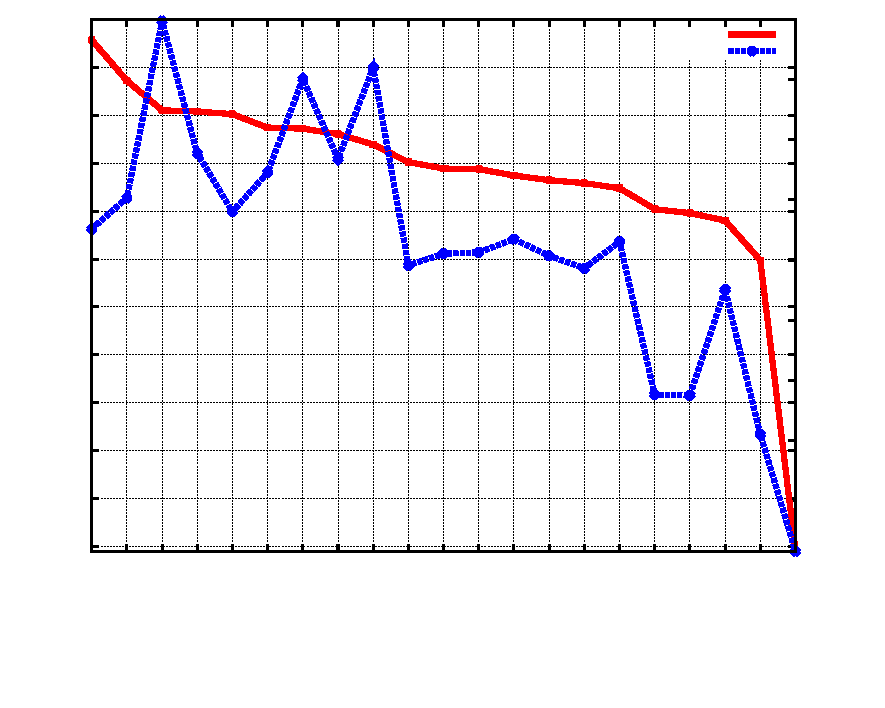
\includegraphics{plots/doc-X.pdf}}%
    \gplfronttext
  \end{picture}%
\endgroup
}
\caption{Doc classification.}
\label{fig:doc}
\end{figure}

\subsection{RNN \& Sequence Tagging}

\paragraph{Model}

\begin{align*}
  \mathbf{h}_i &= f(\mathbf{h}_{i-1}\mathbf{W}+\mathbf{w}_i\cdot\mathbf{U}+\mathbf{b})\\
  \mathbf{y}_i &= \text{softmax}(\mathbf{h}_i\mathbf{V}+\mathbf{c})
\end{align*}

\paragraph{Data}

\paragraph{Approach}

\begin{itemize}[noitemsep,leftmargin=0.6cm]
  \item (1): TL-AM with Glove-100d word embeddings and 5\% of the original training data as train data; (2) the same with 30\% of the original training data as train data. In both cases, dev and test follow the original train splits \cite{Eger:2017}.
  \item (3,4) Same as (1) and (2) but with 300d Levy word embeddings \cite{Levy:2014}.
  \item (5,6): POS with Glove-100d word embeddings and 5\% and 30\%, respectively, of the train data of a pre-determined train/dev/test split (13k/13k/178k tokens). Dev and test are fixed in both cases.
\end{itemize}

\paragraph{Results}

\begin{figure}[!htb]
\centering
\scalebox{0.5}{
% GNUPLOT: LaTeX picture with Postscript
\begingroup
  \makeatletter
  \providecommand\color[2][]{%
    \GenericError{(gnuplot) \space\space\space\@spaces}{%
      Package color not loaded in conjunction with
      terminal option `colourtext'%
    }{See the gnuplot documentation for explanation.%
    }{Either use 'blacktext' in gnuplot or load the package
      color.sty in LaTeX.}%
    \renewcommand\color[2][]{}%
  }%
  \providecommand\includegraphics[2][]{%
    \GenericError{(gnuplot) \space\space\space\@spaces}{%
      Package graphicx or graphics not loaded%
    }{See the gnuplot documentation for explanation.%
    }{The gnuplot epslatex terminal needs graphicx.sty or graphics.sty.}%
    \renewcommand\includegraphics[2][]{}%
  }%
  \providecommand\rotatebox[2]{#2}%
  \@ifundefined{ifGPcolor}{%
    \newif\ifGPcolor
    \GPcolortrue
  }{}%
  \@ifundefined{ifGPblacktext}{%
    \newif\ifGPblacktext
    \GPblacktexttrue
  }{}%
  % define a \g@addto@macro without @ in the name:
  \let\gplgaddtomacro\g@addto@macro
  % define empty templates for all commands taking text:
  \gdef\gplbacktext{}%
  \gdef\gplfronttext{}%
  \makeatother
  \ifGPblacktext
    % no textcolor at all
    \def\colorrgb#1{}%
    \def\colorgray#1{}%
  \else
    % gray or color?
    \ifGPcolor
      \def\colorrgb#1{\color[rgb]{#1}}%
      \def\colorgray#1{\color[gray]{#1}}%
      \expandafter\def\csname LTw\endcsname{\color{white}}%
      \expandafter\def\csname LTb\endcsname{\color{black}}%
      \expandafter\def\csname LTa\endcsname{\color{black}}%
      \expandafter\def\csname LT0\endcsname{\color[rgb]{1,0,0}}%
      \expandafter\def\csname LT1\endcsname{\color[rgb]{0,1,0}}%
      \expandafter\def\csname LT2\endcsname{\color[rgb]{0,0,1}}%
      \expandafter\def\csname LT3\endcsname{\color[rgb]{1,0,1}}%
      \expandafter\def\csname LT4\endcsname{\color[rgb]{0,1,1}}%
      \expandafter\def\csname LT5\endcsname{\color[rgb]{1,1,0}}%
      \expandafter\def\csname LT6\endcsname{\color[rgb]{0,0,0}}%
      \expandafter\def\csname LT7\endcsname{\color[rgb]{1,0.3,0}}%
      \expandafter\def\csname LT8\endcsname{\color[rgb]{0.5,0.5,0.5}}%
    \else
      % gray
      \def\colorrgb#1{\color{black}}%
      \def\colorgray#1{\color[gray]{#1}}%
      \expandafter\def\csname LTw\endcsname{\color{white}}%
      \expandafter\def\csname LTb\endcsname{\color{black}}%
      \expandafter\def\csname LTa\endcsname{\color{black}}%
      \expandafter\def\csname LT0\endcsname{\color{black}}%
      \expandafter\def\csname LT1\endcsname{\color{black}}%
      \expandafter\def\csname LT2\endcsname{\color{black}}%
      \expandafter\def\csname LT3\endcsname{\color{black}}%
      \expandafter\def\csname LT4\endcsname{\color{black}}%
      \expandafter\def\csname LT5\endcsname{\color{black}}%
      \expandafter\def\csname LT6\endcsname{\color{black}}%
      \expandafter\def\csname LT7\endcsname{\color{black}}%
      \expandafter\def\csname LT8\endcsname{\color{black}}%
    \fi
  \fi
  \setlength{\unitlength}{0.0500bp}%
  \begin{picture}(8502.00,6802.00)%
    \gplgaddtomacro\gplbacktext{%
      \csname LTb\endcsname%
      \put(592,1988){\makebox(0,0)[r]{\strut{} 77}}%
      \csname LTb\endcsname%
      \put(592,2618){\makebox(0,0)[r]{\strut{} 80}}%
      \csname LTb\endcsname%
      \put(592,3248){\makebox(0,0)[r]{\strut{} 83}}%
      \csname LTb\endcsname%
      \put(592,3878){\makebox(0,0)[r]{\strut{} 86}}%
      \csname LTb\endcsname%
      \put(592,4509){\makebox(0,0)[r]{\strut{} 89}}%
      \csname LTb\endcsname%
      \put(592,5139){\makebox(0,0)[r]{\strut{} 92}}%
      \csname LTb\endcsname%
      \put(592,5769){\makebox(0,0)[r]{\strut{} 95}}%
      \csname LTb\endcsname%
      \put(592,6399){\makebox(0,0)[r]{\strut{} 98}}%
      \csname LTb\endcsname%
      \put(688,1408){\rotatebox{-270}{\makebox(0,0)[r]{\strut{}\relu}}}%
      \csname LTb\endcsname%
      \put(1151,1408){\rotatebox{-270}{\makebox(0,0)[r]{\strut{}\lrelua}}}%
      \csname LTb\endcsname%
      \put(1615,1408){\rotatebox{-270}{\makebox(0,0)[r]{\strut{}\swish}}}%
      \csname LTb\endcsname%
      \put(2078,1408){\rotatebox{-270}{\makebox(0,0)[r]{\strut{}\pentan}}}%
      \csname LTb\endcsname%
      \put(2541,1408){\rotatebox{-270}{\makebox(0,0)[r]{\strut{}\lrelub}}}%
      \csname LTb\endcsname%
      \put(3004,1408){\rotatebox{-270}{\makebox(0,0)[r]{\strut{}\arctid}}}%
      \csname LTb\endcsname%
      \put(3468,1408){\rotatebox{-270}{\makebox(0,0)[r]{\strut{}\elu}}}%
      \csname LTb\endcsname%
      \put(3931,1408){\rotatebox{-270}{\makebox(0,0)[r]{\strut{}\minsin}}}%
      \csname LTb\endcsname%
      \put(4394,1408){\rotatebox{-270}{\makebox(0,0)[r]{\strut{}\maxtanh}}}%
      \csname LTb\endcsname%
      \put(4857,1408){\rotatebox{-270}{\makebox(0,0)[r]{\strut{}\mytanh}}}%
      \csname LTb\endcsname%
      \put(5321,1408){\rotatebox{-270}{\makebox(0,0)[r]{\strut{}\mysin}}}%
      \csname LTb\endcsname%
      \put(5784,1408){\rotatebox{-270}{\makebox(0,0)[r]{\strut{}\maxsig}}}%
      \csname LTb\endcsname%
      \put(6247,1408){\rotatebox{-270}{\makebox(0,0)[r]{\strut{}\selu}}}%
      \csname LTb\endcsname%
      \put(6710,1408){\rotatebox{-270}{\makebox(0,0)[r]{\strut{}\linear}}}%
      \csname LTb\endcsname%
      \put(7174,1408){\rotatebox{-270}{\makebox(0,0)[r]{\strut{}\sigmoid}}}%
      \csname LTb\endcsname%
      \put(7637,1408){\rotatebox{-270}{\makebox(0,0)[r]{\strut{}\cosid}}}%
      \put(7733,1534){\makebox(0,0)[l]{\strut{} 30}}%
      \put(7733,2259){\makebox(0,0)[l]{\strut{} 40}}%
      \put(7733,2984){\makebox(0,0)[l]{\strut{} 50}}%
      \put(7733,3709){\makebox(0,0)[l]{\strut{} 60}}%
      \put(7733,4434){\makebox(0,0)[l]{\strut{} 70}}%
      \put(7733,5159){\makebox(0,0)[l]{\strut{} 80}}%
      \put(7733,5884){\makebox(0,0)[l]{\strut{} 90}}%
      \put(7733,6609){\makebox(0,0)[l]{\strut{} 100}}%
      \put(128,4056){\rotatebox{-270}{\makebox(0,0){\strut{}Score}}}%
    }%
    \gplgaddtomacro\gplfronttext{%
      \csname LTb\endcsname%
      \put(6902,6466){\makebox(0,0)[r]{\strut{}\best}}%
      \csname LTb\endcsname%
      \put(6902,6306){\makebox(0,0)[r]{\strut{}\avg}}%
    }%
    \gplbacktext
    \put(0,0){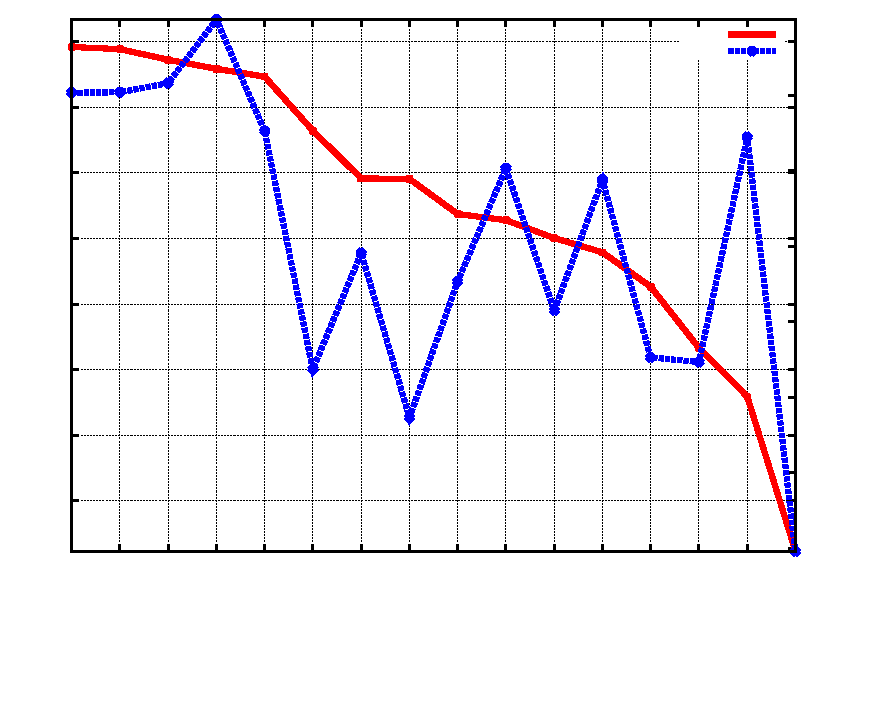
\includegraphics{plots/seq-X.pdf}}%
    \gplfronttext
  \end{picture}%
\endgroup
}
\caption{Sequence tagging.}
\label{fig:seq}
\end{figure}

\paragraph{LSTM vs.\ RNN}

\begin{align*}
  \mathbf{f}_t &= \sigma([\mathbf{h}_{t-1};\mathbf{x}_t]\cdot \mathbf{W}_f),\\
  \mathbf{i}_t &= \sigma([\mathbf{h}_{t-1};\mathbf{x}_t]\cdot \mathbf{W}_i),\\
  \mathbf{o}_t &= \sigma([\mathbf{h}_{t-1};\mathbf{x}_t]\cdot \mathbf{W}_o)\\
  \mathbf{c}_t &= \mathbf{f}_t\odot \mathbf{c}_{t-1}+\mathbf{i}_t\odot\tau([\mathbf{h}_{t-1};\mathbf{x}_t]\cdot \mathbf{W}_c)\\
  \mathbf{h}_t &= \mathbf{o}_t\odot \tau(\mathbf{c}_t),
\end{align*}

\section{Analysis \& Discussion}

\paragraph{Winner statistics}

\begin{table}[!htb]
  \centering
  \begin{tabular}{ll}
  \toprule
    \best{} & \pentan{} (6), \swish{} (6), \\
    & \elu{} (4), \relu{} (4), \lrelua{} (4)\\
    \avg{} & \pentan{} (16), \mytanh{} (13)\\
    & \mysin{} (10) \\
  \bottomrule
  \end{tabular}
  \caption{Top-3 winner statistics. In brackets: number of times within top-3, keeping only functions with four or more top-3 rankings.}
  \label{table:topN}
\end{table}

\paragraph{Influence of hyperparameters}

\begin{align}\label{eq:regression}
  y = \alpha_l\cdot\log(n_l)+\alpha_d\cdot d+\cdots
\end{align}

\section{Concluding remarks}

\bibliography{emnlp2018-2}

\bibliographystyle{acl_natbib}

\appendix

\section{Supplemental Material}

\begin{figure}[!htb]
\scalebox{0.5}{
% GNUPLOT: LaTeX picture with Postscript
\begingroup
  \makeatletter
  \providecommand\color[2][]{%
    \GenericError{(gnuplot) \space\space\space\@spaces}{%
      Package color not loaded in conjunction with
      terminal option `colourtext'%
    }{See the gnuplot documentation for explanation.%
    }{Either use 'blacktext' in gnuplot or load the package
      color.sty in LaTeX.}%
    \renewcommand\color[2][]{}%
  }%
  \providecommand\includegraphics[2][]{%
    \GenericError{(gnuplot) \space\space\space\@spaces}{%
      Package graphicx or graphics not loaded%
    }{See the gnuplot documentation for explanation.%
    }{The gnuplot epslatex terminal needs graphicx.sty or graphics.sty.}%
    \renewcommand\includegraphics[2][]{}%
  }%
  \providecommand\rotatebox[2]{#2}%
  \@ifundefined{ifGPcolor}{%
    \newif\ifGPcolor
    \GPcolortrue
  }{}%
  \@ifundefined{ifGPblacktext}{%
    \newif\ifGPblacktext
    \GPblacktexttrue
  }{}%
  % define a \g@addto@macro without @ in the name:
  \let\gplgaddtomacro\g@addto@macro
  % define empty templates for all commands taking text:
  \gdef\gplbacktext{}%
  \gdef\gplfronttext{}%
  \makeatother
  \ifGPblacktext
    % no textcolor at all
    \def\colorrgb#1{}%
    \def\colorgray#1{}%
  \else
    % gray or color?
    \ifGPcolor
      \def\colorrgb#1{\color[rgb]{#1}}%
      \def\colorgray#1{\color[gray]{#1}}%
      \expandafter\def\csname LTw\endcsname{\color{white}}%
      \expandafter\def\csname LTb\endcsname{\color{black}}%
      \expandafter\def\csname LTa\endcsname{\color{black}}%
      \expandafter\def\csname LT0\endcsname{\color[rgb]{1,0,0}}%
      \expandafter\def\csname LT1\endcsname{\color[rgb]{0,1,0}}%
      \expandafter\def\csname LT2\endcsname{\color[rgb]{0,0,1}}%
      \expandafter\def\csname LT3\endcsname{\color[rgb]{1,0,1}}%
      \expandafter\def\csname LT4\endcsname{\color[rgb]{0,1,1}}%
      \expandafter\def\csname LT5\endcsname{\color[rgb]{1,1,0}}%
      \expandafter\def\csname LT6\endcsname{\color[rgb]{0,0,0}}%
      \expandafter\def\csname LT7\endcsname{\color[rgb]{1,0.3,0}}%
      \expandafter\def\csname LT8\endcsname{\color[rgb]{0.5,0.5,0.5}}%
    \else
      % gray
      \def\colorrgb#1{\color{black}}%
      \def\colorgray#1{\color[gray]{#1}}%
      \expandafter\def\csname LTw\endcsname{\color{white}}%
      \expandafter\def\csname LTb\endcsname{\color{black}}%
      \expandafter\def\csname LTa\endcsname{\color{black}}%
      \expandafter\def\csname LT0\endcsname{\color{black}}%
      \expandafter\def\csname LT1\endcsname{\color{black}}%
      \expandafter\def\csname LT2\endcsname{\color{black}}%
      \expandafter\def\csname LT3\endcsname{\color{black}}%
      \expandafter\def\csname LT4\endcsname{\color{black}}%
      \expandafter\def\csname LT5\endcsname{\color{black}}%
      \expandafter\def\csname LT6\endcsname{\color{black}}%
      \expandafter\def\csname LT7\endcsname{\color{black}}%
      \expandafter\def\csname LT8\endcsname{\color{black}}%
    \fi
  \fi
  \setlength{\unitlength}{0.0500bp}%
  \begin{picture}(8502.00,6802.00)%
    \gplgaddtomacro\gplbacktext{%
      \csname LTb\endcsname%
      \put(528,320){\makebox(0,0)[r]{\strut{}-1}}%
      \csname LTb\endcsname%
      \put(528,949){\makebox(0,0)[r]{\strut{}-0.8}}%
      \csname LTb\endcsname%
      \put(528,1578){\makebox(0,0)[r]{\strut{}-0.6}}%
      \csname LTb\endcsname%
      \put(528,2207){\makebox(0,0)[r]{\strut{}-0.4}}%
      \csname LTb\endcsname%
      \put(528,2836){\makebox(0,0)[r]{\strut{}-0.2}}%
      \csname LTb\endcsname%
      \put(528,3465){\makebox(0,0)[r]{\strut{} 0}}%
      \csname LTb\endcsname%
      \put(528,4093){\makebox(0,0)[r]{\strut{} 0.2}}%
      \csname LTb\endcsname%
      \put(528,4722){\makebox(0,0)[r]{\strut{} 0.4}}%
      \csname LTb\endcsname%
      \put(528,5351){\makebox(0,0)[r]{\strut{} 0.6}}%
      \csname LTb\endcsname%
      \put(528,5980){\makebox(0,0)[r]{\strut{} 0.8}}%
      \csname LTb\endcsname%
      \put(528,6609){\makebox(0,0)[r]{\strut{} 1}}%
      \csname LTb\endcsname%
      \put(624,160){\makebox(0,0){\strut{}-4}}%
      \csname LTb\endcsname%
      \put(1573,160){\makebox(0,0){\strut{}-3}}%
      \csname LTb\endcsname%
      \put(2521,160){\makebox(0,0){\strut{}-2}}%
      \csname LTb\endcsname%
      \put(3470,160){\makebox(0,0){\strut{}-1}}%
      \csname LTb\endcsname%
      \put(4419,160){\makebox(0,0){\strut{} 0}}%
      \csname LTb\endcsname%
      \put(5367,160){\makebox(0,0){\strut{} 1}}%
      \csname LTb\endcsname%
      \put(6316,160){\makebox(0,0){\strut{} 2}}%
      \csname LTb\endcsname%
      \put(7264,160){\makebox(0,0){\strut{} 3}}%
      \csname LTb\endcsname%
      \put(8213,160){\makebox(0,0){\strut{} 4}}%
    }%
    \gplgaddtomacro\gplfronttext{%
      \csname LTb\endcsname%
      \put(7478,943){\makebox(0,0)[r]{\strut{}\sigmoid(x)}}%
      \csname LTb\endcsname%
      \put(7478,783){\makebox(0,0)[r]{\strut{}\pentan(x)}}%
      \csname LTb\endcsname%
      \put(7478,623){\makebox(0,0)[r]{\strut{}\mytanh(x)}}%
      \csname LTb\endcsname%
      \put(7478,463){\makebox(0,0)[r]{\strut{}\mysin(x)}}%
    }%
    \gplbacktext
    \put(0,0){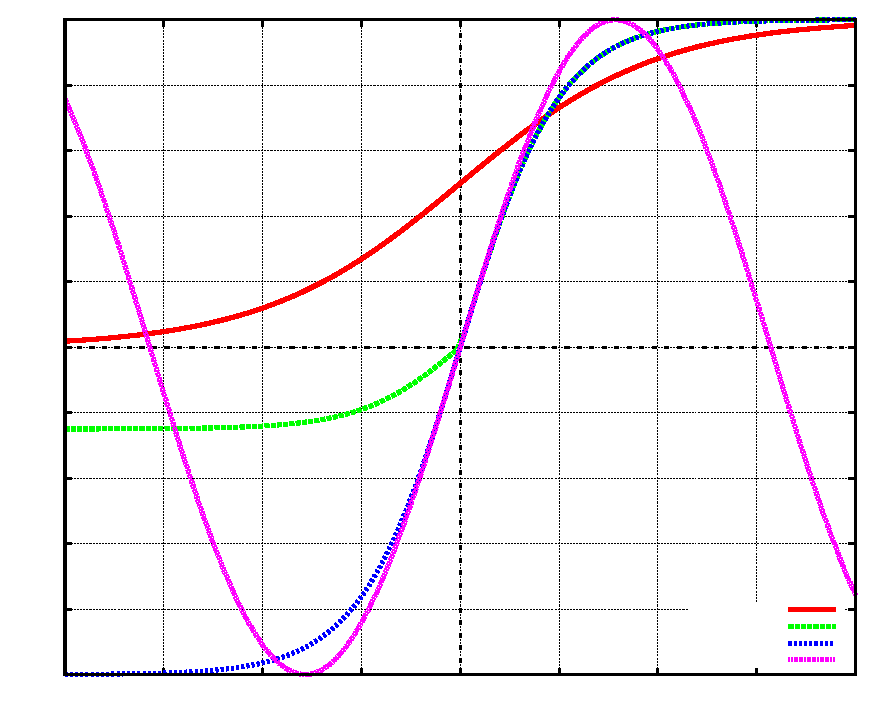
\includegraphics{plots/saturating-X.pdf}}%
    \gplfronttext
  \end{picture}%
\endgroup
}
\scalebox{0.5}{
% GNUPLOT: LaTeX picture with Postscript
\begingroup
  \makeatletter
  \providecommand\color[2][]{%
    \GenericError{(gnuplot) \space\space\space\@spaces}{%
      Package color not loaded in conjunction with
      terminal option `colourtext'%
    }{See the gnuplot documentation for explanation.%
    }{Either use 'blacktext' in gnuplot or load the package
      color.sty in LaTeX.}%
    \renewcommand\color[2][]{}%
  }%
  \providecommand\includegraphics[2][]{%
    \GenericError{(gnuplot) \space\space\space\@spaces}{%
      Package graphicx or graphics not loaded%
    }{See the gnuplot documentation for explanation.%
    }{The gnuplot epslatex terminal needs graphicx.sty or graphics.sty.}%
    \renewcommand\includegraphics[2][]{}%
  }%
  \providecommand\rotatebox[2]{#2}%
  \@ifundefined{ifGPcolor}{%
    \newif\ifGPcolor
    \GPcolortrue
  }{}%
  \@ifundefined{ifGPblacktext}{%
    \newif\ifGPblacktext
    \GPblacktexttrue
  }{}%
  % define a \g@addto@macro without @ in the name:
  \let\gplgaddtomacro\g@addto@macro
  % define empty templates for all commands taking text:
  \gdef\gplbacktext{}%
  \gdef\gplfronttext{}%
  \makeatother
  \ifGPblacktext
    % no textcolor at all
    \def\colorrgb#1{}%
    \def\colorgray#1{}%
  \else
    % gray or color?
    \ifGPcolor
      \def\colorrgb#1{\color[rgb]{#1}}%
      \def\colorgray#1{\color[gray]{#1}}%
      \expandafter\def\csname LTw\endcsname{\color{white}}%
      \expandafter\def\csname LTb\endcsname{\color{black}}%
      \expandafter\def\csname LTa\endcsname{\color{black}}%
      \expandafter\def\csname LT0\endcsname{\color[rgb]{1,0,0}}%
      \expandafter\def\csname LT1\endcsname{\color[rgb]{0,1,0}}%
      \expandafter\def\csname LT2\endcsname{\color[rgb]{0,0,1}}%
      \expandafter\def\csname LT3\endcsname{\color[rgb]{1,0,1}}%
      \expandafter\def\csname LT4\endcsname{\color[rgb]{0,1,1}}%
      \expandafter\def\csname LT5\endcsname{\color[rgb]{1,1,0}}%
      \expandafter\def\csname LT6\endcsname{\color[rgb]{0,0,0}}%
      \expandafter\def\csname LT7\endcsname{\color[rgb]{1,0.3,0}}%
      \expandafter\def\csname LT8\endcsname{\color[rgb]{0.5,0.5,0.5}}%
    \else
      % gray
      \def\colorrgb#1{\color{black}}%
      \def\colorgray#1{\color[gray]{#1}}%
      \expandafter\def\csname LTw\endcsname{\color{white}}%
      \expandafter\def\csname LTb\endcsname{\color{black}}%
      \expandafter\def\csname LTa\endcsname{\color{black}}%
      \expandafter\def\csname LT0\endcsname{\color{black}}%
      \expandafter\def\csname LT1\endcsname{\color{black}}%
      \expandafter\def\csname LT2\endcsname{\color{black}}%
      \expandafter\def\csname LT3\endcsname{\color{black}}%
      \expandafter\def\csname LT4\endcsname{\color{black}}%
      \expandafter\def\csname LT5\endcsname{\color{black}}%
      \expandafter\def\csname LT6\endcsname{\color{black}}%
      \expandafter\def\csname LT7\endcsname{\color{black}}%
      \expandafter\def\csname LT8\endcsname{\color{black}}%
    \fi
  \fi
  \setlength{\unitlength}{0.0500bp}%
  \begin{picture}(8502.00,6802.00)%
    \gplgaddtomacro\gplbacktext{%
      \csname LTb\endcsname%
      \put(336,320){\makebox(0,0)[r]{\strut{}-4}}%
      \csname LTb\endcsname%
      \put(336,1218){\makebox(0,0)[r]{\strut{}-3}}%
      \csname LTb\endcsname%
      \put(336,2117){\makebox(0,0)[r]{\strut{}-2}}%
      \csname LTb\endcsname%
      \put(336,3015){\makebox(0,0)[r]{\strut{}-1}}%
      \csname LTb\endcsname%
      \put(336,3914){\makebox(0,0)[r]{\strut{} 0}}%
      \csname LTb\endcsname%
      \put(336,4812){\makebox(0,0)[r]{\strut{} 1}}%
      \csname LTb\endcsname%
      \put(336,5711){\makebox(0,0)[r]{\strut{} 2}}%
      \csname LTb\endcsname%
      \put(336,6609){\makebox(0,0)[r]{\strut{} 3}}%
      \csname LTb\endcsname%
      \put(432,160){\makebox(0,0){\strut{}-3}}%
      \csname LTb\endcsname%
      \put(1729,160){\makebox(0,0){\strut{}-2}}%
      \csname LTb\endcsname%
      \put(3026,160){\makebox(0,0){\strut{}-1}}%
      \csname LTb\endcsname%
      \put(4323,160){\makebox(0,0){\strut{} 0}}%
      \csname LTb\endcsname%
      \put(5619,160){\makebox(0,0){\strut{} 1}}%
      \csname LTb\endcsname%
      \put(6916,160){\makebox(0,0){\strut{} 2}}%
      \csname LTb\endcsname%
      \put(8213,160){\makebox(0,0){\strut{} 3}}%
    }%
    \gplgaddtomacro\gplfronttext{%
      \csname LTb\endcsname%
      \put(7478,1103){\makebox(0,0)[r]{\strut{}\relu(x)}}%
      \csname LTb\endcsname%
      \put(7478,943){\makebox(0,0)[r]{\strut{}\swish(x)}}%
      \csname LTb\endcsname%
      \put(7478,783){\makebox(0,0)[r]{\strut{}\maxsig(x)}}%
      \csname LTb\endcsname%
      \put(7478,623){\makebox(0,0)[r]{\strut{}\cosid(x)}}%
      \csname LTb\endcsname%
      \put(7478,463){\makebox(0,0)[r]{\strut{}\minsin(x)}}%
    }%
    \gplbacktext
    \put(0,0){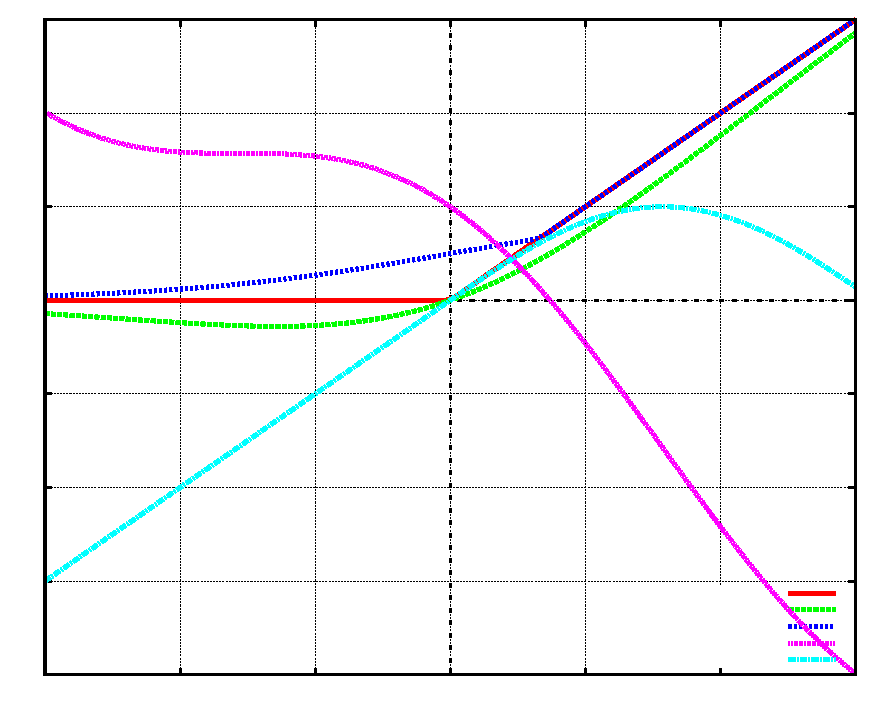
\includegraphics{plots/non-saturating1-X.pdf}}%
    \gplfronttext
  \end{picture}%
\endgroup

}
\caption{Several activation functions.}
\label{fig:saturating}
\end{figure}

\begin{figure}[!htb]
\scalebox{0.5}{
% GNUPLOT: LaTeX picture with Postscript
\begingroup
  \makeatletter
  \providecommand\color[2][]{%
    \GenericError{(gnuplot) \space\space\space\@spaces}{%
      Package color not loaded in conjunction with
      terminal option `colourtext'%
    }{See the gnuplot documentation for explanation.%
    }{Either use 'blacktext' in gnuplot or load the package
      color.sty in LaTeX.}%
    \renewcommand\color[2][]{}%
  }%
  \providecommand\includegraphics[2][]{%
    \GenericError{(gnuplot) \space\space\space\@spaces}{%
      Package graphicx or graphics not loaded%
    }{See the gnuplot documentation for explanation.%
    }{The gnuplot epslatex terminal needs graphicx.sty or graphics.sty.}%
    \renewcommand\includegraphics[2][]{}%
  }%
  \providecommand\rotatebox[2]{#2}%
  \@ifundefined{ifGPcolor}{%
    \newif\ifGPcolor
    \GPcolortrue
  }{}%
  \@ifundefined{ifGPblacktext}{%
    \newif\ifGPblacktext
    \GPblacktexttrue
  }{}%
  % define a \g@addto@macro without @ in the name:
  \let\gplgaddtomacro\g@addto@macro
  % define empty templates for all commands taking text:
  \gdef\gplbacktext{}%
  \gdef\gplfronttext{}%
  \makeatother
  \ifGPblacktext
    % no textcolor at all
    \def\colorrgb#1{}%
    \def\colorgray#1{}%
  \else
    % gray or color?
    \ifGPcolor
      \def\colorrgb#1{\color[rgb]{#1}}%
      \def\colorgray#1{\color[gray]{#1}}%
      \expandafter\def\csname LTw\endcsname{\color{white}}%
      \expandafter\def\csname LTb\endcsname{\color{black}}%
      \expandafter\def\csname LTa\endcsname{\color{black}}%
      \expandafter\def\csname LT0\endcsname{\color[rgb]{1,0,0}}%
      \expandafter\def\csname LT1\endcsname{\color[rgb]{0,1,0}}%
      \expandafter\def\csname LT2\endcsname{\color[rgb]{0,0,1}}%
      \expandafter\def\csname LT3\endcsname{\color[rgb]{1,0,1}}%
      \expandafter\def\csname LT4\endcsname{\color[rgb]{0,1,1}}%
      \expandafter\def\csname LT5\endcsname{\color[rgb]{1,1,0}}%
      \expandafter\def\csname LT6\endcsname{\color[rgb]{0,0,0}}%
      \expandafter\def\csname LT7\endcsname{\color[rgb]{1,0.3,0}}%
      \expandafter\def\csname LT8\endcsname{\color[rgb]{0.5,0.5,0.5}}%
    \else
      % gray
      \def\colorrgb#1{\color{black}}%
      \def\colorgray#1{\color[gray]{#1}}%
      \expandafter\def\csname LTw\endcsname{\color{white}}%
      \expandafter\def\csname LTb\endcsname{\color{black}}%
      \expandafter\def\csname LTa\endcsname{\color{black}}%
      \expandafter\def\csname LT0\endcsname{\color{black}}%
      \expandafter\def\csname LT1\endcsname{\color{black}}%
      \expandafter\def\csname LT2\endcsname{\color{black}}%
      \expandafter\def\csname LT3\endcsname{\color{black}}%
      \expandafter\def\csname LT4\endcsname{\color{black}}%
      \expandafter\def\csname LT5\endcsname{\color{black}}%
      \expandafter\def\csname LT6\endcsname{\color{black}}%
      \expandafter\def\csname LT7\endcsname{\color{black}}%
      \expandafter\def\csname LT8\endcsname{\color{black}}%
    \fi
  \fi
  \setlength{\unitlength}{0.0500bp}%
  \begin{picture}(8502.00,6802.00)%
    \gplgaddtomacro\gplbacktext{%
      \csname LTb\endcsname%
      \put(336,320){\makebox(0,0)[r]{\strut{}-2}}%
      \csname LTb\endcsname%
      \put(336,1218){\makebox(0,0)[r]{\strut{}-1}}%
      \csname LTb\endcsname%
      \put(336,2117){\makebox(0,0)[r]{\strut{} 0}}%
      \csname LTb\endcsname%
      \put(336,3015){\makebox(0,0)[r]{\strut{} 1}}%
      \csname LTb\endcsname%
      \put(336,3914){\makebox(0,0)[r]{\strut{} 2}}%
      \csname LTb\endcsname%
      \put(336,4812){\makebox(0,0)[r]{\strut{} 3}}%
      \csname LTb\endcsname%
      \put(336,5711){\makebox(0,0)[r]{\strut{} 4}}%
      \csname LTb\endcsname%
      \put(336,6609){\makebox(0,0)[r]{\strut{} 5}}%
      \csname LTb\endcsname%
      \put(432,160){\makebox(0,0){\strut{}-3}}%
      \csname LTb\endcsname%
      \put(1729,160){\makebox(0,0){\strut{}-2}}%
      \csname LTb\endcsname%
      \put(3026,160){\makebox(0,0){\strut{}-1}}%
      \csname LTb\endcsname%
      \put(4323,160){\makebox(0,0){\strut{} 0}}%
      \csname LTb\endcsname%
      \put(5619,160){\makebox(0,0){\strut{} 1}}%
      \csname LTb\endcsname%
      \put(6916,160){\makebox(0,0){\strut{} 2}}%
      \csname LTb\endcsname%
      \put(8213,160){\makebox(0,0){\strut{} 3}}%
    }%
    \gplgaddtomacro\gplfronttext{%
      \csname LTb\endcsname%
      \put(7478,1103){\makebox(0,0)[r]{\strut{}\arctid(x)}}%
      \csname LTb\endcsname%
      \put(7478,943){\makebox(0,0)[r]{\strut{}\maxtanh(x)}}%
      \csname LTb\endcsname%
      \put(7478,783){\makebox(0,0)[r]{\strut{}\lrelua(x)}}%
      \csname LTb\endcsname%
      \put(7478,623){\makebox(0,0)[r]{\strut{}\lrelub(x)}}%
      \csname LTb\endcsname%
      \put(7478,463){\makebox(0,0)[r]{\strut{}\elu(x)}}%
    }%
    \gplbacktext
    \put(0,0){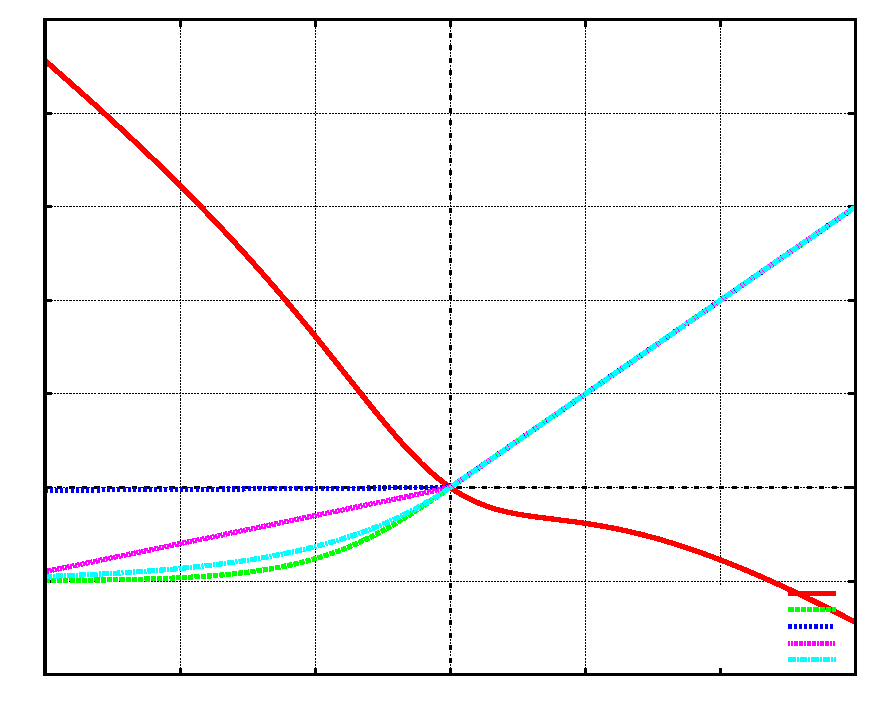
\includegraphics{plots/non-saturating2-X.pdf}}%
    \gplfronttext
  \end{picture}%
\endgroup
}
\scalebox{0.5}{
% GNUPLOT: LaTeX picture with Postscript
\begingroup
  \makeatletter
  \providecommand\color[2][]{%
    \GenericError{(gnuplot) \space\space\space\@spaces}{%
      Package color not loaded in conjunction with
      terminal option `colourtext'%
    }{See the gnuplot documentation for explanation.%
    }{Either use 'blacktext' in gnuplot or load the package
      color.sty in LaTeX.}%
    \renewcommand\color[2][]{}%
  }%
  \providecommand\includegraphics[2][]{%
    \GenericError{(gnuplot) \space\space\space\@spaces}{%
      Package graphicx or graphics not loaded%
    }{See the gnuplot documentation for explanation.%
    }{The gnuplot epslatex terminal needs graphicx.sty or graphics.sty.}%
    \renewcommand\includegraphics[2][]{}%
  }%
  \providecommand\rotatebox[2]{#2}%
  \@ifundefined{ifGPcolor}{%
    \newif\ifGPcolor
    \GPcolortrue
  }{}%
  \@ifundefined{ifGPblacktext}{%
    \newif\ifGPblacktext
    \GPblacktexttrue
  }{}%
  % define a \g@addto@macro without @ in the name:
  \let\gplgaddtomacro\g@addto@macro
  % define empty templates for all commands taking text:
  \gdef\gplbacktext{}%
  \gdef\gplfronttext{}%
  \makeatother
  \ifGPblacktext
    % no textcolor at all
    \def\colorrgb#1{}%
    \def\colorgray#1{}%
  \else
    % gray or color?
    \ifGPcolor
      \def\colorrgb#1{\color[rgb]{#1}}%
      \def\colorgray#1{\color[gray]{#1}}%
      \expandafter\def\csname LTw\endcsname{\color{white}}%
      \expandafter\def\csname LTb\endcsname{\color{black}}%
      \expandafter\def\csname LTa\endcsname{\color{black}}%
      \expandafter\def\csname LT0\endcsname{\color[rgb]{1,0,0}}%
      \expandafter\def\csname LT1\endcsname{\color[rgb]{0,1,0}}%
      \expandafter\def\csname LT2\endcsname{\color[rgb]{0,0,1}}%
      \expandafter\def\csname LT3\endcsname{\color[rgb]{1,0,1}}%
      \expandafter\def\csname LT4\endcsname{\color[rgb]{0,1,1}}%
      \expandafter\def\csname LT5\endcsname{\color[rgb]{1,1,0}}%
      \expandafter\def\csname LT6\endcsname{\color[rgb]{0,0,0}}%
      \expandafter\def\csname LT7\endcsname{\color[rgb]{1,0.3,0}}%
      \expandafter\def\csname LT8\endcsname{\color[rgb]{0.5,0.5,0.5}}%
    \else
      % gray
      \def\colorrgb#1{\color{black}}%
      \def\colorgray#1{\color[gray]{#1}}%
      \expandafter\def\csname LTw\endcsname{\color{white}}%
      \expandafter\def\csname LTb\endcsname{\color{black}}%
      \expandafter\def\csname LTa\endcsname{\color{black}}%
      \expandafter\def\csname LT0\endcsname{\color{black}}%
      \expandafter\def\csname LT1\endcsname{\color{black}}%
      \expandafter\def\csname LT2\endcsname{\color{black}}%
      \expandafter\def\csname LT3\endcsname{\color{black}}%
      \expandafter\def\csname LT4\endcsname{\color{black}}%
      \expandafter\def\csname LT5\endcsname{\color{black}}%
      \expandafter\def\csname LT6\endcsname{\color{black}}%
      \expandafter\def\csname LT7\endcsname{\color{black}}%
      \expandafter\def\csname LT8\endcsname{\color{black}}%
    \fi
  \fi
  \setlength{\unitlength}{0.0500bp}%
  \begin{picture}(8502.00,6802.00)%
    \gplgaddtomacro\gplbacktext{%
      \csname LTb\endcsname%
      \put(336,320){\makebox(0,0)[r]{\strut{}-3}}%
      \csname LTb\endcsname%
      \put(336,1218){\makebox(0,0)[r]{\strut{}-2}}%
      \csname LTb\endcsname%
      \put(336,2117){\makebox(0,0)[r]{\strut{}-1}}%
      \csname LTb\endcsname%
      \put(336,3015){\makebox(0,0)[r]{\strut{} 0}}%
      \csname LTb\endcsname%
      \put(336,3914){\makebox(0,0)[r]{\strut{} 1}}%
      \csname LTb\endcsname%
      \put(336,4812){\makebox(0,0)[r]{\strut{} 2}}%
      \csname LTb\endcsname%
      \put(336,5711){\makebox(0,0)[r]{\strut{} 3}}%
      \csname LTb\endcsname%
      \put(336,6609){\makebox(0,0)[r]{\strut{} 4}}%
      \csname LTb\endcsname%
      \put(432,160){\makebox(0,0){\strut{}-3}}%
      \csname LTb\endcsname%
      \put(1665,160){\makebox(0,0){\strut{}-2}}%
      \csname LTb\endcsname%
      \put(2898,160){\makebox(0,0){\strut{}-1}}%
      \csname LTb\endcsname%
      \put(4131,160){\makebox(0,0){\strut{} 0}}%
      \csname LTb\endcsname%
      \put(5363,160){\makebox(0,0){\strut{} 1}}%
      \csname LTb\endcsname%
      \put(6596,160){\makebox(0,0){\strut{} 2}}%
      \csname LTb\endcsname%
      \put(7829,160){\makebox(0,0){\strut{} 3}}%
      \put(7925,320){\makebox(0,0)[l]{\strut{}-3}}%
      \put(7925,1218){\makebox(0,0)[l]{\strut{}-2}}%
      \put(7925,2117){\makebox(0,0)[l]{\strut{}-1}}%
      \put(7925,3015){\makebox(0,0)[l]{\strut{} 0}}%
      \put(7925,3914){\makebox(0,0)[l]{\strut{} 1}}%
      \put(7925,4812){\makebox(0,0)[l]{\strut{} 2}}%
      \put(7925,5711){\makebox(0,0)[l]{\strut{} 3}}%
      \put(7925,6609){\makebox(0,0)[l]{\strut{} 4}}%
    }%
    \gplgaddtomacro\gplfronttext{%
      \csname LTb\endcsname%
      \put(7094,783){\makebox(0,0)[r]{\strut{}\selu(x)}}%
      \csname LTb\endcsname%
      \put(7094,623){\makebox(0,0)[r]{\strut{}\linear(x)}}%
      \csname LTb\endcsname%
      \put(7094,463){\makebox(0,0)[r]{\strut{}\cube(x)/10}}%
    }%
    \gplbacktext
    \put(0,0){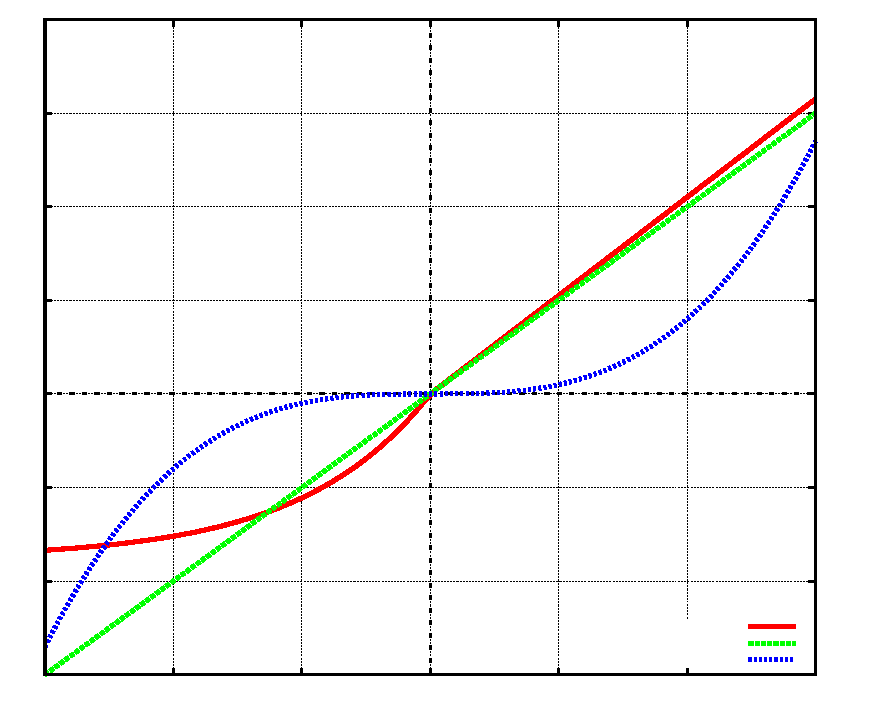
\includegraphics{plots/non-saturating3-X.pdf}}%
    \gplfronttext
  \end{picture}%
\endgroup

}
\caption{Several activation functions.}
\label{fig:nonsaturating}
\end{figure}

\end{document}
